\documentclass[10pt,letterpaper]{article}
\usepackage[utf8]{inputenc}
\usepackage[spanish,english]{babel}
\usepackage{amsmath}
\usepackage{amsfonts}
\usepackage{amssymb}
\usepackage{graphicx}
\usepackage{geometry}
\usepackage{hyperref}
\usepackage{booktabs}
\usepackage{caption}
\usepackage{float}
\usepackage{titlesec}
\usepackage{mathptmx}
\usepackage{enumitem}

\geometry{letterpaper, top=2.5cm, bottom=2.5cm, left=2.5cm, right=2.5cm}
\setlength{\parindent}{1em}
\setlength{\parskip}{6pt}

\titleformat{\section}{\fontsize{12}{14}\selectfont\bfseries}{\thesection.}{0.5em}{}
\titlespacing*{\section}{0pt}{12pt}{4pt}
\titleformat{\subsection}{\fontsize{10}{12}\selectfont\bfseries}{\thesubsection}{0.5em}{}
\titlespacing*{\subsection}{0pt}{10pt}{2pt}
\titleformat{\subsubsection}{\fontsize{10}{12}\selectfont\itshape}{\thesubsubsection}{0.5em}{}
\titlespacing*{\subsubsection}{0pt}{8pt}{2pt}

\captionsetup{font={normalsize}, labelfont=bf, labelsep=colon, justification=centering}
\hypersetup{colorlinks=true, linkcolor=black, citecolor=black, urlcolor=blue}
\pagestyle{empty}

\begin{document}
\thispagestyle{empty}

\begin{center}
    {\fontsize{16}{19}\selectfont\bfseries Desarrollo de una Arquitectura Modular para Modelos Digitales Fenomenol\'ogicos en Python: Validaci\'on, Pruebas y Replicabilidad} \par\vspace{0.8\baselineskip}
    {\fontsize{10}{12}\selectfont Samuel Aguilera$^{a}$} \\
    {\fontsize{9}{11}\selectfont $^{a}$Carrera de Ingenier\'ia Industrial, Universidad Cat\'olica Boliviana ``San Pablo'', Bolivia} \\
    {\fontsize{9}{11}\selectfont \texttt{samuel.aguilera@ucb.edu.bo}} \par\vspace{0.8\baselineskip}
\end{center}

\begin{center}
    {\fontsize{12}{14}\selectfont\bfseries Resumen}
\end{center}

\selectlanguage{spanish}
En este art\'iculo se presenta la arquitectura computacional de un Modelo Digital Fenomenol\'ogico desarrollado en Python, dise\~nado para ser modular, validable en varias capas y replicable en distintas industrias de proceso. El sistema tiene cuatro m\'odulos principales: un n\'ucleo de balances fenomenol\'ogicos, un motor de restricciones de capacidad, un m\'odulo de configuraci\'on externa con validaci\'on autom\'atica y una interfaz de visualizaci\'on en Streamlit. Como caso de validaci\'on, se prob\'o la arquitectura en una planta de Prote\'ina Aislada de Soya (ISP) de $1000\,\text{kg/h}$. Una campa\~na de Monte Carlo de 100,000 corridas sobre el dise\~no inicial dio solo $4.70\%$ de \'exito operativo. Despu\'es de ajustar los equipos cr\'iticos, una segunda campa\~na de 300,000 corridas alcanz\'o $99.88\%$ de \'exito ($3.03\sigma$). Once pruebas unitarias automatizadas verifican la integridad num\'erica del sistema.

\vspace{6pt}
{\fontsize{10}{12}\selectfont\bfseries Palabras Clave:} Modelo Digital, C\'odigo Abierto, Python, Monte Carlo, Simulaci\'on de Procesos.

\vspace{12pt}

\begin{center}
    {\fontsize{12}{14}\selectfont\bfseries Abstract}
\end{center}

\selectlanguage{english}
This paper presents the computational architecture of a Phenomenological Digital Model developed in Python. The design prioritizes modularity, multi-layer validation, and replicability across process industries. The system has four decoupled modules: a phenomenological mass and energy balance kernel, an equipment constraint engine, an external configuration layer with automatic validation, and a Streamlit visualization interface. The architecture is validated through an Isolated Soy Protein (ISP) plant case study at 1,000~kg/h. A Monte Carlo campaign of 100,000 runs on the initial design yielded only 4.70\% success. After resizing the bottleneck equipment, a second campaign of 300,000 runs achieved 99.88\% success (3.03$\sigma$). Eleven automated unit tests verify the system's numerical integrity, and the complete source code is publicly available under MIT license.

\vspace{6pt}
{\fontsize{10}{12}\selectfont\bfseries Keywords:} Digital Model, Open Source, Python, Monte Carlo, Process Simulation.

\selectlanguage{spanish}

\section{Introducci\'on}

Kritzinger et al.~\cite{kritzinger2018digital} definen tres niveles de integraci\'on virtual: \textbf{Modelo Digital} (representaci\'on est\'atica sin intercambio autom\'atico de datos), \textbf{Sombra Digital} (flujo de datos del proceso al modelo en una sola direcci\'on) y \textbf{Gemelo Digital} (flujo bidireccional con control predictivo en tiempo real). La mayor\'ia de los trabajos publicados se enfocan en los dos niveles superiores, pero usan plataformas comerciales que hacen dif\'icil replicarlos de forma independiente~\cite{gil2024survey}. Hace falta una plataforma de c\'odigo abierto para el nivel base de esta jerarqu\'ia: el Modelo Digital fenomenol\'ogico.

Am\'erica Latina, y en particular Bolivia, es una regi\'on importante en la producci\'on de soya. Santa Cruz concentra m\'as del 90\% de la producci\'on nacional, con una industria de derivados (harina, aceite, prote\'ina aislada) en crecimiento. La soya es el cultivo industrial m\'as importante de Bolivia, con m\'as de 1.2 millones de hect\'areas cultivadas~\cite{cao2023}. Sin embargo, el uso de herramientas de simulaci\'on y gemelos digitales en la industria latinoamericana todav\'ia es limitado. Esto se debe a que no hay plataformas accesibles, en espa\~nol y que se puedan replicar sin invertir en software comercial. La arquitectura que se presenta en este trabajo busca reducir ese problema.

Este trabajo presenta una arquitectura computacional de Modelo Digital Fenomenol\'ogico que es modular, replicable y de c\'odigo abierto. El sistema est\'a en el primer nivel de la clasificaci\'on de Kritzinger: no necesita flujo de datos en tiempo real ni infraestructura IoT. Su n\'ucleo usa ecuaciones de conservaci\'on de masa y energ\'ia, no correlaciones emp\'iricas ni modelos de caja negra. Esto hace que el modelo sea interpretable, f\'acil de depurar y se pueda adaptar a otros procesos~\cite{perry2019}.

El art\'iculo est\'a organizado de la siguiente forma. La Secci\'on~2 presenta los trabajos relacionados. La Secci\'on~3 explica la metodolog\'ia de desarrollo. La Secci\'on~4 describe la arquitectura propuesta. La Secci\'on~5 explica los requisitos de replicabilidad. La Secci\'on~6 muestra la verificaci\'on num\'erica con el caso de estudio ISP. La Secci\'on~7 presenta las conclusiones y el trabajo futuro.

\section{Trabajo Relacionado y Comparativa}

\subsection{Frameworks de C\'odigo Abierto}

\textbf{OpenTwins}~\cite{robles2023opentwins} es un framework de c\'odigo abierto para gemelos digitales composicionales basado en Eclipse Ditto, con integraci\'on IoT y visualizaci\'on 3D. Requiere infraestructura Kubernetes y no incluye modelos fenomenol\'ogicos.

\textbf{CoFMPy}~\cite{friedrich2025cofmupy} es un framework en Python para prototipado r\'apido de gemelos digitales usando co-simulaci\'on FMI, permitiendo integrar FMUs con IA. Es la alternativa tecnol\'ogicamente m\'as cercana porque est\'a implementada en Python puro.

\textbf{DT-Forge}~\cite{dtforge2025} propone una arquitectura de seis capas para gemelos con telemetr\'ia en tiempo real, que requiere Docker, MQTT, InfluxDB, MongoDB y Neo4j.

\textbf{UniTwin}~\cite{haussermann2024unitwin} presenta gemelos digitales universales en contenedores Kubernetes con \'enfasis en reconfigurabilidad din\'amica.

\textbf{TumorTwin}~\cite{tumortwin2025} es un framework Python para gemelos digitales personalizados en oncolog\'ia. Al igual que este proyecto, usa Python puro y tiene un dise\~no modular.

\textbf{Udugama et al.}~\cite{udugama2023digital} proponen modelos digitales de varias capas para la industria alimentaria. \textbf{Gamero et al.}~\cite{gamero2024data} presentan el concepto de \textit{Lean Digital Twin} para biorefiner\'ias. \textbf{Verboven et al.}~\cite{verboven2020digital} establecen las bases conceptuales para gemelos digitales en procesamiento de alimentos.

\begin{table}[!ht]
\centering
\caption{Comparativa de Frameworks para Modelos Digitales}
\label{tab:comparativa}
\small
\begin{tabular}{lccccccc}
\toprule
\textbf{Framework} & \textbf{Python} & \textbf{Valid.} & \textbf{Pruebas} & \textbf{Modelo} & \textbf{Nivel} & \textbf{UI} & \textbf{Caso} \\
 & \textbf{puro} & \textbf{Estad.} & \textbf{Unit.} & \textbf{Fenom.} & \textbf{Integr.} & & \textbf{Real} \\
\midrule
Este proyecto & $\checkmark$ & $\checkmark$ & $\checkmark$ & $\checkmark$ & Modelo & $\checkmark$ & $\checkmark$ \\
OpenTwins~\cite{robles2023opentwins} & $\times$ & $\times$ & $\times$ & $\times$ & Gemelo & $\checkmark$ & $\checkmark$ \\
CoFMPy~\cite{friedrich2025cofmupy} & $\checkmark$ & $\times$ & $\times$ & FMU ext. & Sombra & GUI & $\checkmark$ \\
DT-Forge~\cite{dtforge2025} & $\checkmark$ & $\times$ & $\times$ & Opcional & Gemelo & $\times$ & $\times$ \\
UniTwin~\cite{haussermann2024unitwin} & $\times$ & $\times$ & $\times$ & $\times$ & Gemelo & $\checkmark$ & $\times$ \\
TumorTwin~\cite{tumortwin2025} & $\checkmark$ & $\times$ & $\times$ & $\checkmark$ & Modelo & $\times$ & $\checkmark$ \\
\bottomrule
\end{tabular}
\end{table}

Como se muestra en la Tabla~\ref{tab:comparativa}, la mayor\'ia de los frameworks existentes no tienen validaci\'on estad\'istica ni pruebas unitarias automatizadas. Nuestra propuesta es el \'unico framework clasificado como Modelo Digital que incluye las cuatro capas de validaci\'on al mismo tiempo.

\section{Metodolog\'ia}

El desarrollo del modelo digital sigui\'o un proceso iterativo de cuatro etapas:

\begin{enumerate}
    \item \textbf{Formulaci\'on fenomenol\'ogica:} Para cada operaci\'on unitaria del proceso ISP se derivaron balances de materia y energ\'ia a partir de primeros principios (conservaci\'on de masa y primera ley de la termodin\'amica). Las eficiencias nominales se obtuvieron de la literatura especializada~\cite{lusas1995soy,kinsella1979}.
    \item \textbf{Implementaci\'on modular en Python:} Cada etapa se program\'o como una funci\'on independiente (\texttt{calc\_stage\_}\allowbreak\texttt{N}) que recibe las variables de control y los par\'ametros del equipo, y devuelve un diccionario con los resultados del balance. La funci\'on \texttt{run\_process\_}\allowbreak\texttt{model} conecta las etapas en secuencia.
    \item \textbf{Validaci\'on y verificaci\'on por capas:} Se implementaron tres niveles: (i) validaci\'on de rangos f\'isicos en los par\'ametros de entrada, (ii) once pruebas unitarias que verifican la consistencia num\'erica, y (iii) verificaci\'on del cierre del balance de masa global (error $<0.1\%$).
    \item \textbf{An\'alisis estoc\'astico de robustez:} Se ejecutaron campa\~nas de Monte Carlo para evaluar el comportamiento del sistema cuando las 19 variables de control var\'ian simult\'aneamente. Los cuellos de botella se identificaron mediante el an\'alisis de frecuencias de falla.
\end{enumerate}

\begin{figure}[!ht]
\centering
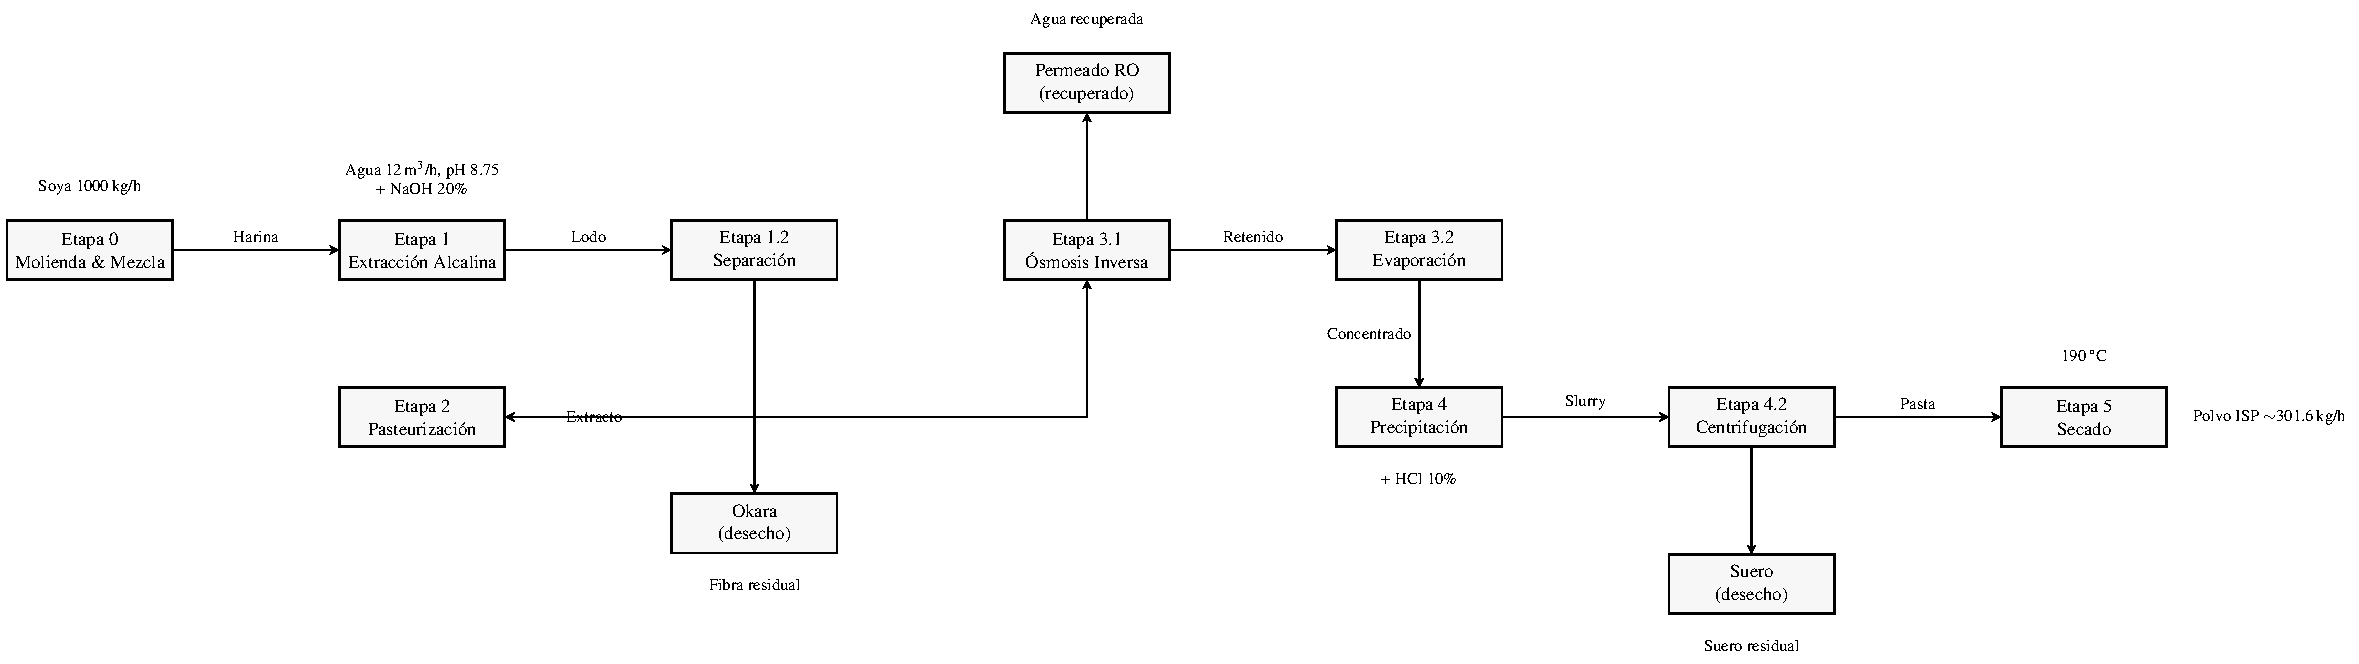
\includegraphics[width=0.85\textwidth]{figures/diagrama_flujo.pdf}
\caption{Diagrama de flujo del proceso ISP con las seis etapas principales.}
\label{fig:diagrama}
\end{figure}

\section{Arquitectura del Modelo Digital}

El sistema est\'a compuesto por cuatro m\'odulos computacionales en el paquete \texttt{core/} y un m\'odulo de interfaz, todos desarrollados en Python 3.10+. Los m\'odulos se comunican entre s\'i mediante diccionarios con una estructura definida.

\subsection{Vista General de M\'odulos}

\begin{itemize}
    \item \texttt{core/equipment\_specs.py} --- Configuraci\'on de equipo. Contiene \texttt{EQUIPMENT\_SPEC\_}\allowbreak\texttt{DEFAULTS} (capacidades nominales), \texttt{EQUIPMENT\_SPEC\_}\allowbreak\texttt{LIMITS} (rangos f\'isicos), \texttt{CAPACITY\_LIMIT\_}\allowbreak\texttt{DEFAULTS} y \texttt{CAPACITY\_LIMIT\_}\allowbreak\texttt{BOUNDS} (factores de seguridad). Las funciones \texttt{validate\_equipment\_}\allowbreak\texttt{specs} y \texttt{validate\_capacity\_}\allowbreak\texttt{limits} revisan los valores autom\'aticamente.
    \item \texttt{core/stage\_equations.py} --- N\'ucleo fenomenol\'ogico. Las funciones \texttt{calc\_stage\_N} resuelven balances de materia y energ\'ia por etapa; los diccionarios \texttt{CONTROL\_}\allowbreak\texttt{LIMITS} y \texttt{KPI\_SPECS}; y \texttt{run\_process\_}\allowbreak\texttt{model} coordina la ejecuci\'on, validaci\'on y cierre del balance.
    \item \texttt{core/equipment\_}\allowbreak\texttt{constraints.py} --- Motor de restricciones. \texttt{evaluate\_capacity\_}\allowbreak\texttt{constraints} compara la carga con la capacidad del equipo. \texttt{enforce\_}\allowbreak\texttt{capacity\_}\allowbreak\texttt{constraints} lanza \texttt{Equipment}\allowbreak\texttt{CapacityError} si hay violaci\'on.
    \item \texttt{core/process\_model.py} --- Soporte de historial. Proporciona \texttt{ControlLog} (un buffer circular de 1000 puntos) y \texttt{build\_snapshot} para organizar controles, especificaciones y resultados.
    \item \texttt{app.py} --- Interfaz en Streamlit. Incluye un bucle de simulaci\'on con paso temporal configurable, inercia de primer orden y visualizaci\'on en tiempo real de KPIs y alarmas.
    \item \texttt{tests/} --- Once pruebas unitarias distribuidas en tres archivos diferentes.
\end{itemize}

\subsection{Configuraci\'on Externalizada y Validaci\'on}

Todos los par\'ametros del proceso est\'an definidos como constantes en los m\'odulos, con validaci\'on autom\'atica en tres capas: valores nominales, l\'imites f\'isicos y l\'imites operativos. Cada variable de control $u_j$ tiene un rango operativo $[u_{j,\min}, u_{j,\max}]$:

\begin{align}
u_j \in \mathbb{R}, \quad |u_j| < \infty, \quad u_{j,\min} \leq u_j \leq u_{j,\max} \quad \forall j \label{eq:validation}
\end{align}

\subsection{N\'ucleo Fenomenol\'ogico}

Cada etapa modela los balances de materia y energ\'ia usando ecuaciones algebraicas. Tambi\'en incluye funciones de penalizaci\'on cuando las condiciones se desv\'ian de los valores nominales, un factor de p\'erdida operativa ($F_{\text{LOSS}}=2\%$ por etapa) y mapas de eficiencia emp\'iricos.

\subsubsection{Etapa 0: Molienda y Mezcla}

\begin{equation}
\dot{m}_{0} = \dot{m}_{\text{soya}} + \rho_w Q_w \label{eq:stage0_mass}
\end{equation}

\subsubsection{Etapa 1: Lixiviaci\'on Alcalina}

\begin{align}
\dot{m}_{\text{prot}} &= \eta_{\text{ext}} \, X_{\text{prot}} \, \dot{m}_{\text{soya}} \label{eq:stage1_extract} \\
\dot{m}_{\text{okara}} &= \frac{\dot{m}_{\text{soya}} \,(1 - \eta_{\text{ext}} X_{\text{prot}})}{1 - H_{\text{okara}}} \label{eq:stage1_okara} \\
\dot{m}_{\text{ext}} &= \dot{m}_0 - \dot{m}_{\text{okara}} \label{eq:stage1_extract_flow}
\end{align}

donde $\eta_{\text{ext}}$ es modulada por funciones continuas que penalizan desviaciones de pH, temperatura, tiempo de residencia y relaci\'on s\'olido--l\'iquido.

\subsubsection{Etapa 2: Pasteurizaci\'on HTST}

\begin{align}
\dot{Q}_{\text{HX}} &= \dot{m}_{\text{ext}} \, C_{p,\text{ext}} \, (T_{\text{out}} - T_{\text{in}}) \label{eq:stage2_energy} \\
A_{\text{HX}} &= \frac{\dot{Q}_{\text{HX}}}{U \, \Delta T_{\text{lm}}} \label{eq:stage2_area}
\end{align}

\subsubsection{Etapa 3: Concentraci\'on (OI + Evaporaci\'on)}

La preconcentraci\'on por \'osmosis inversa sigue un modelo simplificado de presi\'on transmembrana. El evaporador al vac\'io remueve el agua remanente:

\begin{align}
\dot{m}_{\text{perm}} &= f(\Delta P, \dot{m}_{\text{ext}}) \label{eq:stage3_ro} \\
\dot{Q}_{\text{ev}} &= \lambda \, \dot{m}_{\text{vap}} = U_{\text{ev}} \, A_{\text{ev}} \, \Delta T_{\text{ev}} \label{eq:stage3_evap}
\end{align}

\subsubsection{Etapa 4: Precipitaci\'on Isoel\'ectrica y Centrifugaci\'on}

\begin{align}
\dot{m}_{\text{ppt}} &= \eta_{\text{ppt}} \, \dot{m}_{\text{prot,4}} \label{eq:stage4_ppt} \\
\dot{m}_{\text{ppt,h\'umedo}} &= \frac{\dot{m}_{\text{ppt}}}{1 - H_{\text{pasta}}} \label{eq:stage4_paste}
\end{align}

\subsubsection{Etapa 5: Secado por Atomizaci\'on}

\begin{align}
\dot{m}_{\text{powder}} &= \dot{m}_{\text{ppt}} \, \frac{1 - X_{\text{moist,in}}}{1 - X_{\text{moist,out}}} \label{eq:stage5_mass} \\
\dot{Q}_{\text{dry}} &= \dot{m}_{\text{air}} \, C_{p,\text{air}} \, (T_{\text{in}} - T_{\text{out}}) + \lambda \, \dot{m}_{\text{evap}} \label{eq:stage5_energy}
\end{align}

\subsubsection{Inercia Din\'amica}

La respuesta temporal sigue una ecuaci\'on diferencial de primer orden:

\begin{equation}
y[k+1] = y[k] + \bigl( u[k] - y[k] \bigr) \bigl( 1 - e^{-\Delta t / \tau} \bigr) \label{eq:inertia_discrete}
\end{equation}

\subsection{Motor de Restricciones}

Las restricciones de capacidad se escriben como inecuaciones que comparan la carga solicitada con la capacidad disponible, ajustada por factores de seguridad $f_s$:

\begin{align}
V_{\text{TK}} &\leq V_{\text{TK,max}} \cdot f_{s,\text{TK}} \label{eq:constr_tank} \\
\dot{Q}_{\text{HX}} &\leq A_{\text{HX,max}} \cdot U \cdot \Delta T_{\text{lm}} \cdot f_{s,\text{HX}} \label{eq:constr_hx} \\
\dot{m}_{\text{vap}} &\leq \dot{m}_{\text{vap,max}} \cdot f_{s,\text{EV}} \label{eq:constr_evap}
\end{align}

Cuando hay una violaci\'on, el sistema genera una alarma con un c\'odigo, un mensaje y una recomendaci\'on. Esto separa la detecci\'on de fallas de la l\'ogica del proceso.

\subsection{Sistema de Pruebas Unitarias}

Once pruebas automatizadas verifican los siguientes aspectos: consistencia del balance de materia, rendimientos no negativos, comparaci\'on del caso base con valores de referencia ($\pm0.5\%$), detecci\'on de bloqueos de capacidad y validaci\'on de rangos de control.

\section{Requisitos de Replicabilidad}

La adaptaci\'on a un nuevo proceso requiere tres pasos independientes:

\begin{enumerate}
    \item \textbf{Mapeo de equipos:} Crear \texttt{EQUIPMENT\_SPEC\_}\allowbreak\texttt{DEFAULTS} (capacidades) y \texttt{CAPACITY\_LIMIT\_}\allowbreak\texttt{DEFAULTS} (factores de seguridad). La funci\'on \texttt{validate\_equipment\_}\allowbreak\texttt{specs} revisa los rangos f\'isicos.
    \item \textbf{Implementaci\'on de balances:} Escribir una funci\'on \texttt{stage\_n}\allowbreak\texttt{(controls,}\allowbreak\texttt{ specs)} para cada operaci\'on unitaria. Si no se necesita un modelo detallado, se pueden usar factores de rendimiento emp\'iricos.
    \item \textbf{Definici\'on de controles:} Definir \texttt{CONTROL\_}\allowbreak\texttt{LIMITS} con los rangos operativos. La funci\'on \texttt{validate\_}\allowbreak\texttt{controls} asegura que ning\'un valor fuera de especificaci\'on llegue al modelo.
\end{enumerate}

\section{Verificaci\'on Num\'erica: Caso de Estudio ISP}

\subsection{Verificaci\'on del Balance de Materia}

Con los par\'ametros nominales ($F_{\text{soya}} = 1000\,\text{kg/h}$, $Q_{\text{agua}} = 12\,\text{m}^3/\text{h}$, pH 8.75, $T_{\text{pasteur}} = 80\,^\circ\text{C}$, pH$_{\text{precip}} = 4.5$, $T_{\text{secado}} = 190\,^\circ\text{C}$), el modelo produce:

\begin{itemize}
    \item Eficiencia de extracci\'on: $88.0\%$
    \item Prote\'ina precipitada: $292.3\,\text{kg/h}$
    \item Polvo proteico final: $301.6\,\text{kg/h}$ ($286.5\,\text{kg/h}$ de prote\'ina)
    \item Rendimiento global de prote\'ina: $76.40\%$
    \item Humedad residual del polvo: $5.0\%$
    \item Cierre del balance de masa: error $<0.1\%$
\end{itemize}

\subsection{Diagn\'ostico Estoc\'astico del Dise\~no Base}

Se ejecutaron 10 lotes de Monte Carlo (100,000 corridas en total) sobre el dise\~no base. Solo el $4.70\%$ de las corridas fueron exitosas ($\sigma = \pm 0.18\%$, IC 95\%: $[4.59\%, 4.81\%]$). Los cuellos de botella identificados fueron: tanque de lixiviaci\'on TK-101 ($78.23\%$ de las fallas), tanque de agua TK-100 ($69.50\%$), evaporador EV-301 ($57.06\%$) y pasteurizador HX-201 ($40.69\%$).

\subsection{Redimensionamiento y Validaci\'on Final}

Despu\'es de ajustar los equipos cr\'iticos (Tabla~\ref{tab:restrictions}), se ejecut\'o una campa\~na de 30 lotes (300,000 corridas) con rangos ampliados ($\pm20\%$ en alimentaci\'on, $\pm25\%$ en flujo de agua). Los resultados fueron:

\begin{itemize}
    \item \textbf{Tasa de \'exito:} $99.88\%$ (299,633/300,000)
    \item \textbf{Desviaci\'on est\'andar:} $\pm 0.026\%$, IC 95\%: $[99.87\%, 99.89\%]$
    \item \textbf{Nivel Sigma:} $Z = 3.03\sigma$ ($\sim1200$ DPMO)
    \item \textbf{Fallas residuales:} Solo \texttt{STAGE1\_TANK\_CAPACITY} en $0.12\%$
\end{itemize}

\begin{table}[!ht]
\centering
\caption{L\'imites de Capacidad (Configuraci\'on Optimizada)}
\label{tab:restrictions}
\small
\begin{tabular}{lcc}
\toprule
Restricci\'on & Variable & L\'imite M\'aximo \\
\midrule
TK-100 & Capacidad Geom\'etrica & $22.0\,\text{m}^3$ \\
TK-101 & Capacidad Geom\'etrica & $35.0\,\text{m}^3$ \\
HX-201 & \'Area de Intercambio & $68.5\,\text{m}^2$ \\
EV-301 & Capacidad Evaporativa & $16.0\,\text{m}^3/\text{h}$ \\
CF-401 & Caudal Hidr\'aulico & $10.0\,\text{m}^3/\text{h}$ \\
SD-501 & Capacidad Evaporativa & $1000\,\text{kg/h}$ \\
\bottomrule
\end{tabular}
\end{table}

\begin{figure}[!ht]
\centering
\includegraphics[width=0.8\textwidth]{figures/monte_carlo_dist.pdf}
\caption{Distribuci\'on de tasas de \'exito por lote en la campa\~na optimizada.}
\label{fig:mc_dist}
\end{figure}

\subsection{An\'alisis Energ\'etico}

La \'osmosis inversa elimina $2718.3\,\text{kg/h}$ de agua en fase l\'iquida usando solo $8.5\,\text{kW}$ el\'ectricos. Esto reduce la carga t\'ermica del evaporador en $836.2\,\text{kW}$ ($19.5\%$). El ahorro neto de $827.7\,\text{kW}$ permite recuperar la inversi\'on en la membrana en menos de 1.5 a\~nos.

\begin{table}[!ht]
\centering
\caption{Comparaci\'on Energ\'etica: Sin OI vs Con OI}
\label{tab:energy_comparison}
\small
\begin{tabular}{lcc}
\toprule
Variable & Sin OI & Con OI \\
\midrule
Agua removida evap. ($\text{kg/h}$) & $6841.0$ & $5509.0$ \\
Agua removida OI ($\text{kg/h}$) & $0.0$ & $2718.3$ \\
Potencia T\'ermica Evap. ($\text{kW}$) & $4294.6$ & $3458.4$ \\
Ahorro t\'ermico ($\text{kW}$) & $0.0$ & $836.2\ (19.5\%)$ \\
Potencia El\'ectrica OI ($\text{kW}$) & $0.0$ & $8.5$ \\
Ahorro Neto ($\text{kW}$) & $0.0$ & $827.7$ \\
\bottomrule
\end{tabular}
\end{table}

\section{Conclusiones y Trabajo Futuro}

En este trabajo se present\'o la arquitectura computacional de un Modelo Digital Fenomenol\'ogico dise\~nado para ser replicable en diferentes industrias de proceso. Las caracter\'isticas principales son: (i) configuraci\'on externa con validaci\'on autom\'atica, (ii) ecuaciones independientes para cada etapa, (iii) motor de restricciones separado de la l\'ogica del proceso, y (iv) pruebas unitarias automatizadas.

La aplicaci\'on a una planta de ISP demostr\'o su utilidad pr\'actica. El diagn\'ostico Monte Carlo mejor\'o el dise\~no de $4.70\%$ a $99.88\%$ de \'exito ($3.03\sigma$), y el an\'alisis energ\'etico mostr\'o un ahorro del $19.5\%$ usando \'osmosis inversa. Once pruebas unitarias garantizan la integridad num\'erica, y el c\'odigo completo est\'a publicado bajo licencia MIT.

El c\'odigo fuente completo est\'a disponible en un repositorio p\'ublico bajo licencia MIT. Como trabajo futuro, se proyecta la transici\'on a Sombra Digital con instrumentaci\'on IoT, la composici\'on de m\'ultiples plantas siguiendo el enfoque de OpenTwins y la incorporaci\'on de modelos h\'ibridos de IA para predecir la calidad del producto.

\section*{Agradecimientos}

El autor expresa su m\'as sincero agradecimiento al Ing. Francisco Dilillo (docente de la materia de Procesos Unitarios) por su valioso apoyo y gu\'ia en la realizaci\'on de este trabajo.

\begin{thebibliography}{99}
\footnotesize
\bibitem{kritzinger2018digital} W. Kritzinger et al., ``Digital Twin in manufacturing: A categorical literature review and classification,'' \textit{IFAC-PapersOnLine}, vol.~51, no.~11, pp. 1016--1022, 2018.
\bibitem{gil2024survey} S. Gil et al., ``Survey on open-source digital twin frameworks -- A case study approach,'' \textit{Software Practice and Experience}, vol.~54, no.~6, pp. 929--960, 2024.
\bibitem{robles2023opentwins} J. Robles, C. Mart\'in, and M. D\'iaz, ``OpenTwins: An open-source framework for the development of next-gen compositional digital twins,'' \textit{Computers in Industry}, vol.~152, p. 104007, 2023.
\bibitem{friedrich2025cofmupy} C. Friedrich et al., ``CoFMPy: A Python Framework for Rapid Prototyping of FMI-based Digital Twins,'' in \textit{Proc. 2nd Int. Conf. Engineering Digital Twins (ICEDT)}, 2025.
\bibitem{dtforge2025} DT-Forge Contributors, ``DT-Forge: Domain-agnostic Python framework for digital twin architectures,'' PyPI, 2025.
\bibitem{haussermann2024unitwin} T. H\"au{\ss}ermann et al., ``UniTwin: Pushing Universal Digital Twins Into the Clouds Through Reconfigurable Container Environments,'' \textit{IEEE Internet Computing}, vol.~29, no.~1, pp. 8--15, 2024.
\bibitem{tumortwin2025} TumorTwin Contributors, ``TumorTwin: A Python framework for patient-specific digital twins in oncology,'' arXiv:2505.00670, 2025.
\bibitem{udugama2023digital} I. A. Udugama et al., ``Digital twins in food processing: A conceptual approach to developing multi-layer digital models,'' \textit{Digital Chemical Engineering}, vol.~6, p. 100087, 2023.
\bibitem{gamero2024data} E. Gamero et al., ``Data Management in Biorefineries: Conceptual Thoughts on Lean Digital Twinning,'' \textit{Procedia CIRP}, 2024.
\bibitem{verboven2020digital} P. Verboven, T. Defraeye, A. K. Datta, and B. Nicolai, ``Digital twins of food process operations: the next step for food process models?'' \textit{Current Opinion in Food Science}, vol.~35, pp. 79--87, 2020.
\bibitem{lusas1995soy} E. W. Lusas and M. N. Riaz, ``Soy protein products: processing and use,'' \textit{The Journal of Nutrition}, vol.~125, no.~suppl\_3, pp. 573S--580S, 1995.
\bibitem{kinsella1979} J. E. Kinsella, ``Functional properties of soy proteins,'' \textit{JAOCS}, vol.~56, pp. 242--258, 1979.
\bibitem{kedem1958} O. Kedem and A. Katchalsky, ``Thermodynamic analysis of permeability,'' \textit{BBA}, vol.~27, pp. 229--246, 1958.
\bibitem{roos1995} Y. H. Roos, \textit{Phase Transitions in Foods}, Academic Press, 1995.
\bibitem{perry2019} R. H. Perry and D. W. Green, \textit{Perry's Chemical Engineers' Handbook}, 9th ed., McGraw-Hill, 2019.
\bibitem{iso23247} ISO 23247:2021, ``Digital twin framework for manufacturing,'' ISO, 2021.
\bibitem{opcfoundation2022} OPC Foundation, ``OPC UA Companion Specification for the AAS,'' OPC 30270, 2022.
\bibitem{iec63278} IEC 63278:2023, ``Asset Administration Shell,'' IEC, 2023.
\bibitem{cao2023} C\'amara Agropecuaria del Oriente (CAO), ``Informe Anual de la Soya,'' Santa Cruz, Bolivia, 2023.
\end{thebibliography}

\end{document}
